\documentclass{article}

\usepackage[utf8]{inputenc}
\usepackage[T1]{fontenc}      
\usepackage[francais]{babel}
\usepackage{graphicx}
\usepackage{circuitikz}
\usepackage[squaren, Gray]{SIunits}
\usepackage{sistyle}
\usepackage[autolanguage]{numprint}
\usepackage{pgfplots}
\pgfplotsset{compat=1.9}
\usepackage{amsmath,amssymb,array}
\usepackage[top=2.5cm,bottom=2.5cm,right=2.5cm,left=2.5cm]{geometry}
\usepackage{url} 
\usepackage{tabularx}
\DeclareMathOperator{\dist}{d}
\newenvironment{abstract-fr}
{
	\begin{center}
		\textbf{Résumé} \\[0.5cm]
	\end{center}
}
{}

\newenvironment{abstract-en}
{
	\begin{center}
		\textbf{Summary} \\[0.5cm]
	\end{center}
}
{}
% New command pour la modélisation mécanique, tri à effectuer
\newcommand\fv[1]{{\bf #1}} % free vector
\newcommand\fvd[1]{\dot{\bf #1}} % free vector derivated
\newcommand\fvdd[1]{\ddot{\bf #1}} % free vector derivated
\newcommand\fvr[1]{\mathring{\bf #1}} % free vector relatively derivated
\newcommand\fvrr[1]{\overset{\circ\circ}{\bf #1}} % free vector relatively derivated
\newcommand\uv[1]{{\bf\hat{ #1}}} % unit vector
\newcommand\ui{{\bf\hat{I}}} % unit vector I
\newcommand\uj{{\bf\hat{J}}} % unit vector J
\newcommand\uk{{\bf\hat{K}}} % unit vector K
\newcommand\wrt[2]{\ensuremath{\tensor*[_{ #1}]{ #2}{}}} % With Respect To
\newcommand\wtr[3]{\ensuremath{\tensor*[_{ #1}]{ #2}{^{ #3}}}} % With Two Respect
\newcommand\omegaf{{\bm \omega}}
\newcommand\omegafr{\mathring{\bm \omega}}
\newcommand\omegafd{\dot{\bm \omega}}
\newcommand\omegaft{\tilde{\bm \omega}}
\newcommand\omegaftr{\mathring{\tilde{\bm \omega}}}
\newcommand\omegat{\tilde{\omega}}
\newcommand\omegatd{\tilde{\dot{\omega}}}
\newcommand\ine{{\bf I}}
\newcommand\st{{\bf L}}
\newcommand\pst{{\bf M}}
\newcommand\lm{{\bf N}}
\newcommand\am{{\bf H}}
\newcommand\amd{\dot{\am}}
\newcommand\fo{{\bf F}}
\newcommand\po{\mathcal{P}}
\newcommand\xg{\ensuremath{\fv{R}}}
\newcommand\xgd{\ensuremath{\fvd{R}}}
\newcommand\xgdd{\ensuremath{\fvdd{R}}}
\newcommand\dvec[1]{\dot{\vec{ #1}}}
\newcommand\ddvec[1]{\ddot{\vec{ #1}}}
\newcommand\qp{\dot{q}}
\newcommand\dqp{\Delta \dot{q}}
\usepackage{url} 
\usepackage{hyperref}
\hypersetup{
    colorlinks,
    citecolor=black,
    filecolor=black,
    linkcolor=black,
    urlcolor=black
}

\begin{document}

\section{Dimensionnement de l'électroaimant et de la bobine mobile}
Pour fabriquer notre haut-parleur, nous ne disposions pas d'aimant permanent. Nous avons donc
dû créer un électroaimant à partir d'un matériau ferromagnétique qui nous a été fourni.
Cette section présente dans un premier temps le dimensionnement de cet électroaimant, c'est-à-dire le
nombre de spires choisi, la résistance totale de la bobine, son inductance, etc.

Nous calculerons ensuite, de manière expérimentale, la constante de raideur de la membrane de
notre haut-parleur. A partir de cela et de l'écartement maximal par rapport à sa position d'origine 
(choisi arbitrairement), 
nous pourons calculer la force nécessaire pour déplacer la membrane, et par conséquent, le nombre
de spires nécessaire sur la bobine mobile.

\subsection{Fonctionnement et dimensionnement de la bobine fixe}
Lorsqu'un courant traverse la bobine de cuivre, un champ magnétique est créé.  Nous obtenons 
donc un électroaimant fixe générant le champ nécessaire au déplacement de la seconde bobine. 
C'est cette seconde bobine qui sera responsable du tremblement de la membrane.

\begin{figure}[ht!]
\centering
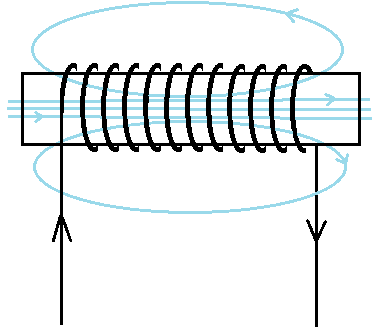
\includegraphics[scale=0.6]{electroaimant.png}
\caption{Modélisation d'un électroaimant}
\label{modélisation de l'électroaimant}
\end{figure}

Le nombre de spires de la bobine fixe, appelons-le $N_1$, a été choisi arbitrairement de manière à produire un
champ magnétique assez fort. Nous avons fixé ce nombre, selon les conseils de notre tuteur, à \numprint{420}. 
Nous allons maintenant calculer les caractéristiques suivantes de notre électroaimant :

\begin{itemize}
	\item Résistance totale de la bobine ;
	\item Champ magnétique induit ;
	\item Inductance.
\end{itemize}

\paragraph{Champ magnétique dans l'entrefer}
Pour céer un champ magnétique plus fort, nous avons réduit l'entrefer de $\unit{7}{\milli\meter}$.
Calculons dans un premier temps le champ magnétique dans l'entrefer de $\unit{7}{\milli\meter}$ en 
utilisant la conservation des flux. Pour ce calcul, nous utilisons l'hypothèse simplificatrice
assez forte que tout le champ se trouve dans l'entrefer.

$$H_e \cdot e = N_1 I \Rightarrow \frac{B_e}{\mu_0 \mu_r} e = N_1 I$$

Pour $N_1 = 420$, l'entrefer $e = \unit{0.007}{\meter}$, $\mu_r = 1.0000004$ la perméabilité magnétique
de l'air et $I = \unit{1}{\ampere}$, on trouve alors :

$B_e = \unit{0.07539825}{\tesla}$

\paragraph{Résistance totale de la bobine}
Pour calculer la résistance totale de la bobine, nous devons connaître la longueur totale de fil de cuivre utilisé.
Pour cela nous utilisons la formule suivante :

$$L{fil} = N_1 \cdot 2\pi r$$  

Où $N_1 = 420$ est le nombre de spires de la bobine fixe, et $r$ est la rayon des spires. Pour
$r = \unit{0.016}{\meter}$, on trouve :

$$L_{fil} = \unit{42.22}{\meter}$$

Il ne nous reste donc plus qu'à multiplier la longueur totale trouvée par la résistance linéique des fils de cuivre
($R_{lin} = \unit{0.18}{\ohm\per\meter}$) :

$$R = L_{fil} \cdot R_{lin} = \unit{7.6}{\ohm}$$

\paragraph{Inductance de la bobine}
Une fois le champ magnétique induit connu, l'inductance dans la bobine peut être très facilement calculée par :

$$L = N_1 \frac{\phi_B}{I}$$

Dans cette formule, il ne nous reste plus qu'à calculer $\phi_B = B \cdot A$ où $A = ab$ est l'aire d'une spire.
On trouve alors :

$L = \unit{0.025468}{\henry}$

\paragraph{Tableau récapitulatif}

\begin{center}
	\begin{tabular}{c|c|c|c|c}
		$N_1$ & $B_e$ & $R$ & $L$ & $L_{fil}$ \\
		\hline
		420 & $\unit{0.07539825}{\tesla}$ & \unit{7.6}{\ohm} & $\unit{0.0254683}{\henry}$ & $\unit{42.22}{\meter}$\\
	\end{tabular}
\end{center}

%Il faut encore recalculer la constante de raideur de la menbranne!

\subsection{Calcul de la constante de raideur de la membrane}
Avant de pouvoir déterminer le nombre de spires de la bobine mouvante, nous avons dû déterminer
expérimentalement la constante de raideur de notre papier pour faire la membrane.
Notre procédure a été la suivante: nous avons suspendu notre membrane, pour ensuite 
déposer un poids dessus, et finalement mesurer l'élongation du matériau.
Nous obtenons ainsi une constante de raideur d'environ \unit {80}{N/m}.

\subsection{Fonctionnement et dimensionnement de la bobine mobile}

\paragraph{Calcul du nombre de spires}
Etant donné que nous disposons d'un amplificateur qui, selon la datasheet, a une puissance de sortie de 
$\unit{2.5}{\watt}$, et que la tension de sortie est de $\unit{15}{\volt}$, nous pouvons trouver le courant
maximal passant dans la bobine mobile:

$$I = \frac{P}{V} = \unit{0.1667}{\ampere}$$

En fonction de la constante de raideur de la membrane trouvée dans la sous-section précédente et de l'écartement
maximal de la membrane par rapport à sa position d'origine (fixé à $d = \unit{0.003}{\meter}$), nous sommes en
mesure de trouver la longueur du fil de la bobine:

$$IL_{fil}B = kx$$
$$L_{fil} = \frac{kx}{IB} = 12.6 m$$

Le fil à notre disposition au laboratoire a un encombrement de $\unit{25.8}{\frac{spires}{cm}}$. Nous otenons 
donc une relation entre $N_2$, le nombre de spires, et $L_{bobine}$, la longueur de la bobine:

$$25.8 = \frac{N_2}{L_{bobine}}$$

En fixant le rayon à \unit{1.7}{mm}, nous pouvons déterminer $N_2$ ainsi que la longueur de la bobine:
$$L_{fil} = N_2 \cdot 2\pi r$$ 
$$N_2 =  \frac{L_{fil}}{2\pi r} = 118$$


\paragraph{Calcul de la résistance totale de la bobine mobile}
Pour calculer la résistance totale de la bobine, il ne nous reste plus qu'à multiplier la longueur de fil trouvée 
précédemment par la résistance linéique du fil de cuivre
($R_{lin} = \unit{0.18}{\ohm\per\meter}$) :

$$R = L_{fil} \cdot R_{lin} = \unit{2.38}{\ohm}$$

\paragraph{Calcul de l'inductance de la bobine mobile}

Une fois le champ magnétique induit connu, l'inductance dans la bobine peut être très facilement calculée par :

$$L = N_2 \frac{\phi_B}{I} = \unit{0.0734}{\henry}$$

\paragraph{Tableau récapitulatif}

\begin{center}
	\begin{tabular}{c|c|c|c}
		$N_2$ & $I$ & $R$ & $L$ \\
		\hline
		 $118$ & $\unit{0.1667}{\ampere}$ & $\unit{2.38}{\ohm}$ & $\unit{0.0734}{\henry}$ \\
	\end{tabular}
\end{center}

\begin{figure}[ht!]
\centering
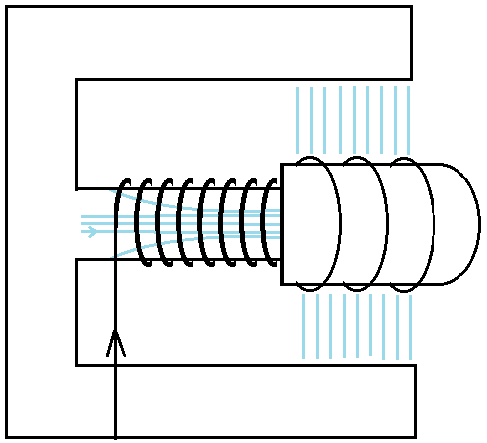
\includegraphics[scale=0.3]{hautparleur.png}
\caption{Vue d'ensemble avec la seconde bobine}
\label{Vue d'ensemble avec la seconde bobine}
\end{figure}

% Just here to fix rapport_prejury.tex
\end{document}